\documentclass[report]{subfiles}

\begin{document}
Below are a short description of each of the different algorithms and techniques which has been used, with focus on the different parameters which can be changed.

\subsection{Gaussian Smoothing}
\label{sec:theoryGaussianSmoothing}
When working on recognizing text in an image, it is desired to get as sharp an image as possible, where all edges of each letter is easily distinctable from the white space around it. This can be achieved by applying a blur to the image, also known as Gaussian Smoothing.\\ 
The kernel will be in the form of a grid, where the height and width will determine how many pixels the smoothing will be applied to, alternatively it can be specified as a radius, depending on what implementation of the algorithm is used.\\
It is therefore desirable to look at both the size of the kernel and the amount of smoothing when trying to get the best setting. In the project, a package called 'EBImage'\footnote{http://www.bioconductor.org/packages/release/bioc/html/EBImage.html} does this for us, the amount of smoothing is called sigma, and the kernel has this default formula:
\begin{lstlisting}
	2*ceiling(3*sigma)+1)
\end{lstlisting}
An example of this effect can be seen at figure~\ref{fig:imgExplainBlur} where an image with and without the blur is illustrated.

\begin{figure}[H]
	\centering
	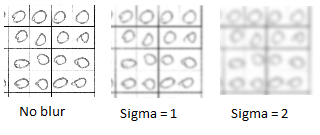
\includegraphics[width=0.5\textwidth]{images/imgBlurDesc}
	\caption{Illustration of the effect of a Gaussian Smoothing}
	\label{fig:imgExplainBlur}
\end{figure}

\subsection{Principal Component Analysis}
\label{sec:theoryPCA}
In the dataset gathered for the project, a lot of the data was similar, or nearly similar, for instance if ten of the same digits were written almost identical. It can therefore speed up the process by a large margin if the dataset is reduced.\\
One technique to reduce the dataset is to run a Principal Component Analysis(PCA) on the data. PCA by itself identifies the data entries with most variance. When the variance is determined, it is then possible to select the data entries with the most variance, which is defined by a parameter. This means that it is possible to run the PCA and get for instance 95\% of the data entries with the most variance, and thereby removing many similar entries and effectively reducing the dataset.

\subsection{K-Means}
\label{sec:theorykMeans}
K-Means

\subsection{KNN}
\label{sec:theoryKNN}
K-Nearest Neighbor(KNN) classification is one of the simplest algorithms used with statistical machine learning. It is a lazy learning, meaning that it does not run its algorithm before test data is provided. It is therefore quickly to train the model, but slow at performing a classification.\\
The idea is to calculate the euclidean distance between all other data entries, and a specific data point. When all the distances are calculated, the one closest to the data point is chosen. An illustration of this can be seen at figure~\ref{fig:knnExp}.

\begin{figure}[H]
	\centering
	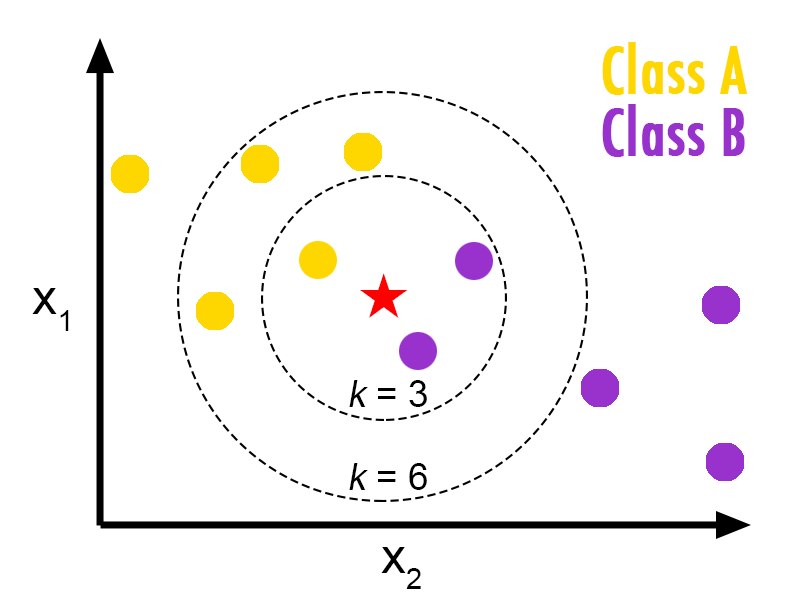
\includegraphics[width=0.35\textwidth]{images/knnExp}
	\caption{Illustration of KNN}
	\label{fig:knnExp}
\end{figure}

The important variable to configure in KNN is the k-value, which specifies how many neighbors is used for determining the result. It is not known beforehand which k-value is the best, one can have an assumption, but testing is needed to figure out the optimal K-value.

\subsection{Random Forest}
\label{sec:theoryRandomForest}
Random Forest\\
Remember: Over fitting of the model and supervised vs unsupervised learning

\end{document}